%%%%%%%%%%%%%%%%%%%%%%%%%%%%%%%%%%%%%%%%%%%%%%%%%%%%%%%%%%%%%%%%%%%%%%%%%%%%%%%%%%%%
\documentclass[a4paper,11pt,oneside]{book} 
\usepackage{styles/CS_report} 
\usepackage{styles/listings-rust}
%%%%%%%%%%%%%%%%%%%%%%%%%%%%%%%%%%%%%%%%%%%%%%%%%%%%%%%%%%%%%%%%%%%%%%%%%%%%%%%%%%%%


%%%%%%%%%%%%%%%%%%%%%%%%%%%%%%%%%%%%%%%%%%%%%%%%%%%%%%%%%%%%%%%%%%%%%%%%%%%%%%%%%%%%
\begin{document}

\captionsetup[figure]{margin=1.5cm,font=small,name={Figure},labelsep=colon}
\captionsetup[table]{margin=1.5cm,font=small,name={Table},labelsep=colon}

\frontmatter

%%%%%%%%%%%%%%%%%%%%%%%%%%%%%%%%%%%%%%%%%%%%%%%%%%%%%%%%%%%%%%%%%%%%%%%%%%%%%%%%
\begin{titlepage}
	\begin{center}
		
\includegraphics[width=3cm]{figures/ufrnlogo.png}\\[0.5cm]
		{\LARGE Universidade Federal do Rio Grande do Norte\\[0.5cm]
		Instituto Metrópole Digital}\\[2cm]
		{\color{blue} \rule{\textwidth}{1pt}}
		\linespread{1.2}\huge {
			Estruturas de Dados Clássicas: Árvore B
		}
		\linespread{1}~\\[2cm]
		%{\color{blue} \rule{\textwidth}{1pt}}
		{\Large
		Bianca Medeiros,
		Gabriel Carvalho,
		Marina Medeiros,
		Vinicius de Lima
		}\\[1cm]

		{\large
		\emph{} Estrutura de Dados Básica II}\\[1cm] % if applicable

		\large Trabalho da Terceira Unidade
		\vfill
		\today
	\end{center}
\end{titlepage}

% -------------------------------------------------------------------
% Contents
% -------------------------------------------------------------------

\tableofcontents

%%%%%%%%%%%%%%%%%%%%%%%%%%%%%%%%%%%%%%%%%%%%%%%%%%%%%%%%%%%%%%%%%%%%%%%%
%%                                                                    %%  
%%  Main chapters and sections of your project                        %%  
%%  Everything from here on needs updates in your own words and works %%
%%                                                                    %%
%%%%%%%%%%%%%%%%%%%%%%%%%%%%%%%%%%%%%%%%%%%%%%%%%%%%%%%%%%%%%%%%%%%%%%%%
\mainmatter
% Read for preparation of document in LaTex 
% Lamport, L. (1986), LATEX: A Document Preparation System, Addison-Wesley.

\chapter{Ambiente computacional}

Todos os testes de performance nesse trabalho foram realizados no seguinte sistema:

\begin{table}[!ht]
	\centering
	\begin{tabular}{llll}
		\toprule
		\multirow{5}{3cm}{Software}
		 & Sistema Operacional          & Arch Linux x86\_64           & \\
		 & Kernel                       & Linux 6.12.8-arch1-1         & \\
		 & Gerenciador de Janelas       & Hyprland (Wayland)           & \\
		 & Terminal                     & Ghostty 1.0.1                & \\
		 & Compilador de C++            & clang 18.1.8                 & \\
		 & Compilador de Rust           & rustc 1.82.0                 & \\
		 & Versão do Cargo              & cargo 1.82.0                 & \\
		 &                              &                              & \\
		\multirow{4}{3cm}{Hardware}
		 & CPU                          & AMD Ryzen 5 5500             & \\
		 & GPU                          & GeForce RTX 4060 Ti          & \\
		 & Driver da GPU                & nvidia (proprietário) 565.77 & \\
		 & Memória RAM                  & 31.24 GiB                    & \\
		 & Armazenamento                & SSD NVMe 2TB                 & \\
		\bottomrule
	\end{tabular}
\end{table}

\noindent

\chapter{Árvore B}
\label{ch:heap} % This how you label a chapter and the key (e.g., ch:into) will be used to refer this chapter ``Introduction'' later in the report. 

% the key ``ch:into'' can be used with command \ref{ch:intor} to refere this Chapter.
% 
\section*{Introdução}
A Árvore B está inclusa na categoria da árvores autobalanceáveis tal qual as árvores AVL e Rubro-Negra, entretanto o que a diferencia destas são seus nós que podem armazenar mais de um valor chave. Idealizada por Rudolf Bayer e Edward Meyers McCreight, esta tem como fim trabalhar com grandes volumes de dados normalmente armazenados em memória secundária(na época, através de discos rígidos magnéticos). 

Devido a isso, sua estratégia conceitual consiste em não carregar todos os dados na memória principal, apenas algumas páginas. E bem como é elucidado na pirâmide de hierarquia de memória, existe uma relação inversamente proporcional entre custo e capacidade de armazenamento de memórias de menor latência.

\begin{figure}[!ht]
	\centering
	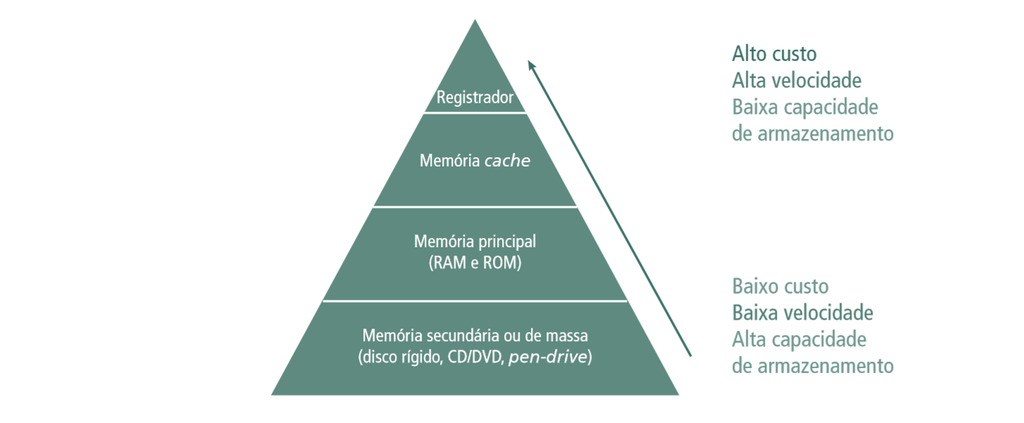
\includegraphics[scale=0.7]{figures/piramide.png}
\end{figure}

Sendo assim, quando se trabalha com um volume significativo de dados é inviável carregar tudo na memória principal. E é tendo isso em mente que a Árvore B carrega apenas partes específicas dos dados na memória, essas partes também são conhecidas como \textbf{páginas}. Sendo assim, essa abordagem visa diminuir a quantidade de operações de entrada e saída da memória secundária.

Ela se assemelha muito com a Árvore Rubro-Negra embora sua altura possa ser significativamente menor devido ao fato dela poder comportar mais de um valor chave por nó. Em suma, toda Árvore B deve ter as seguintes propriedades:

\begin{itemize}
	\item Todas chaves de um nó devem estar ordenadas entre si
	\item Seja ${t \in \mathbb{Z}}$, chamamos \texttt{t} de \textbf{grau mínimo}
		\begin{itemize}
			\item A raiz pode ter entre \texttt{1} e \texttt{2t} chaves
			\item Qualquer outro nó deve ter entre \texttt{t} e \texttt{2t} chaves
			\item Cada nó interno(que não é folha nem raiz) tem entre \texttt{t + 1} e \texttt{2t + 1} filhos
		\end{itemize}
	\item Todo nó tem \texttt{n + 1} ponteiros, em que \texttt{n} é o número de chaves
\end{itemize}

Sintetizando, podemos compreender a Árvore B como algo semelhante à figura abaixo


\begin{figure}[!ht]
	\centering
	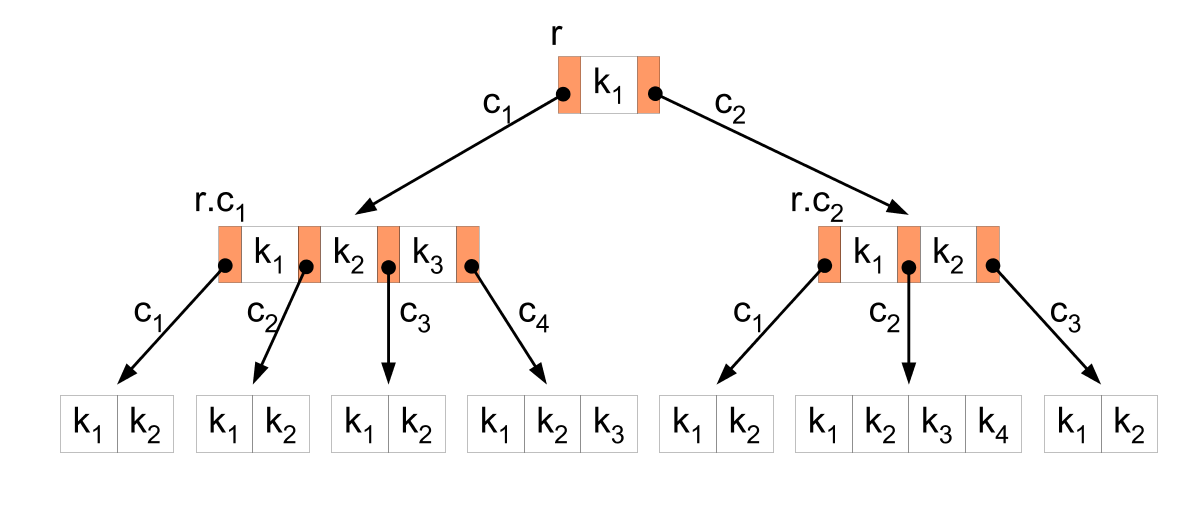
\includegraphics[scale=0.3]{figures/btree.png}
\end{figure}

\section*{Altura}

Embora a altura de uma Árvore B seja muito menor do que uma proporcional Rubro-Negra, essa é muito mais larga. E seja \texttt{h} sua altura e \texttt{n} sua quantidade de elementos, vale que

\begin{equation*}
	h \leq \log_t {\frac{n + 1}{2}}
\end{equation*}

\section*{Busca}

Em uma Árvore Binária de Busca qualquer a operação de busca é uma sequência escolhas binária(esquerda e direita) de qual caminho percorrer até que o elemento seja ou não encontrado. Já nas Árvores B, sua capacidade de armazenar mais de um valor chave por nó faz com que essa escolha binária vire uma escolha \texttt{n+1}-ária, sendo \texttt{n} o número de elementos do nó.

Entretanto, a lógica da busca tem a mesma essência da operação em qualquer BST. Serão feitas apenas as comparações necessárias e quando necessário, a busca seguirá para o nó filho. Ou seja, a busca vai iterar pelo conteúdo do nó(seja valor chave ou ponteiro) em ordem crescente, e sempre vai seguir pelo ponteiro que estiver entre os valores cujo intervalo contém o elemento buscado. Exemplificando:

\begin{figure}[H]
	\centering
	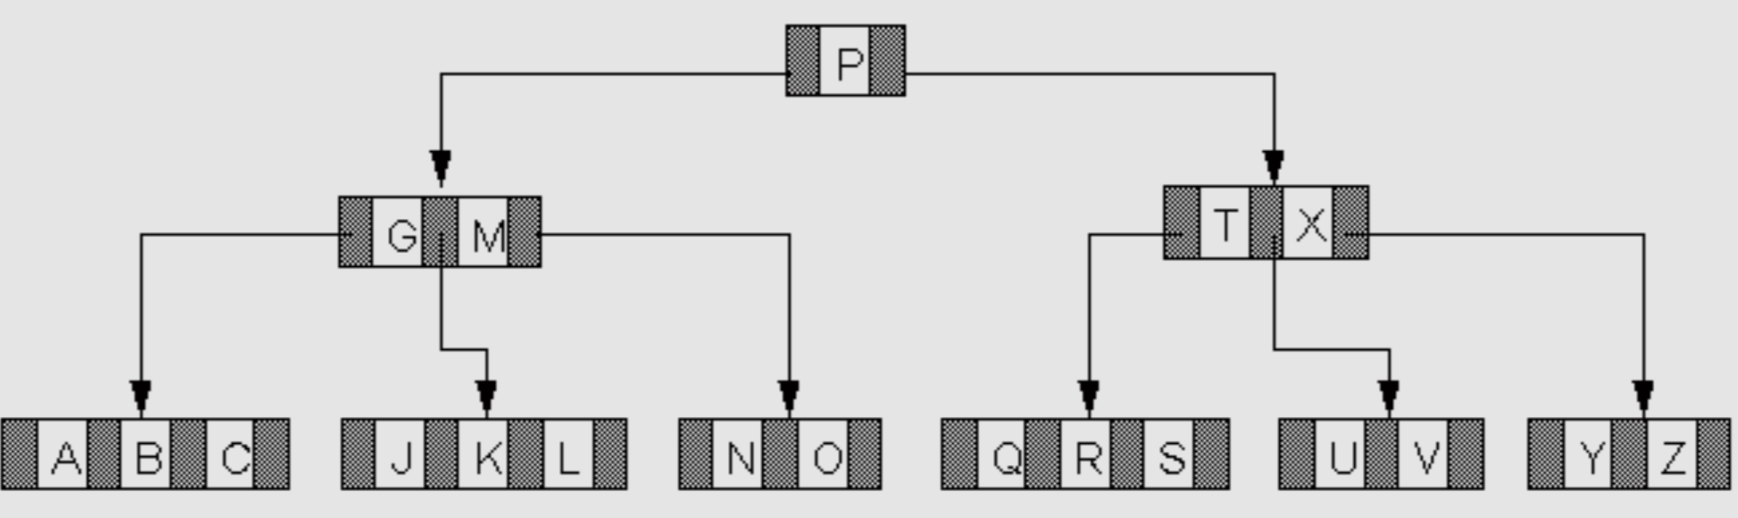
\includegraphics[scale=0.2]{figures/busca-exemplo.png}
\end{figure}

Dada a árvore acima, caso desejamos buscar a chave \textbf{K} o processo seria o seguinte:

\begin{enumerate}
    \item $K \leq P$
    \item Como $K \in (-\infty; P]$, logo seguimos pelo ponteiro à esquerda de $P$
    \item Atualmente em um ponteiro, mas como $K \in [G; M]$, a busca continuará por ele mesmo
    \item $K == K$
\end{enumerate}

\section*{Inserção}
As particularidades da inserção em uma Árvore B acontecem para não violar as propriedades da quantidade de chaves permitidas em um nó. Nos casos em que a inserção causa essa violação, a árvore tem um processo de divisão de nós que ocorre de baixo para cima. Basicamente podemos resumir nos dois exemplos abaixo:

\subsection*{Inserção sem partição}
Esse caso se trata de quando o nó em que se deve ser feita a inserção ainda pode comportar elementos. No exemplo a abaixo a árvore tem ordem 3, ou seja, um nó pode ter entre e 4 chaves por nó.


\begin{figure}[!ht]
	\centering
	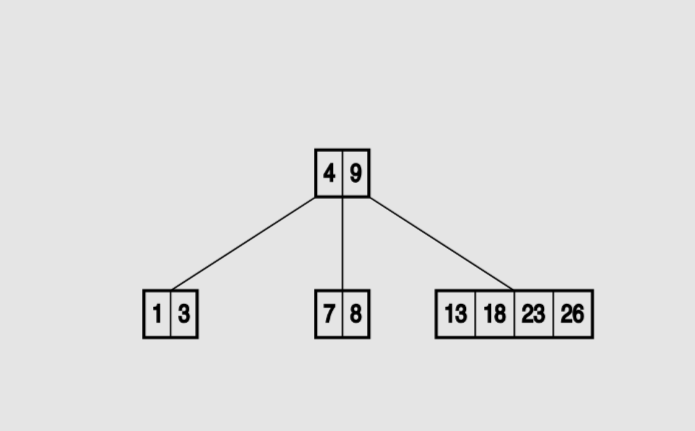
\includegraphics[scale=0.4]{figures/insertion1.png}
\end{figure}

\begin{figure}[!ht]
	\centering
	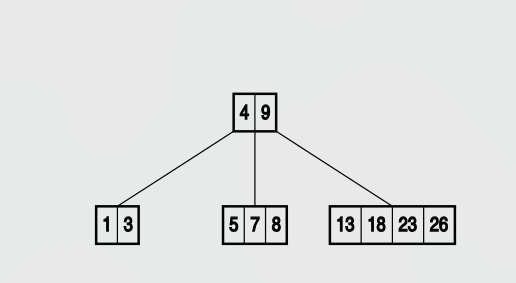
\includegraphics[scale=0.5]{figures/insertion2.png}
\end{figure}

Perceba que após a inserção do 5 nenhuma mudança estrutural significativa aconteceu. E isso ocorre pois o nó que comporta o valor inserido ainda tinha capacidade para adicionar mais um valor nele.

\subsection*{Inserção com partição}

Ainda no mesmo exemplo, agora será feita a inserção de do valor 24, que deve ser alocado no nó mais a direita.

\begin{figure}[H]
	\centering
	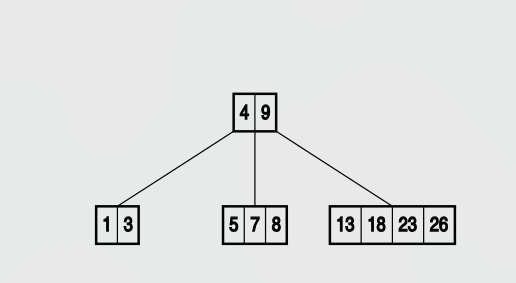
\includegraphics[scale=0.5]{figures/insertion2.png}
\end{figure}

É feita a inserção do valor 24.

\begin{figure}[H]
	\centering
	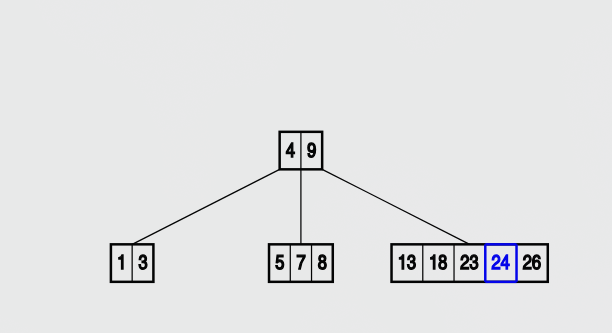
\includegraphics[scale=0.5]{figures/insertion3.png}
\end{figure}

Note que o estrutura acima viola as propriedades da Árvore B de ordem 3, sendo assim ela escolhe o valor médio do nó para ser o pai e reparte a página em dois nós filhos. 

\begin{figure}[H]
	\centering
	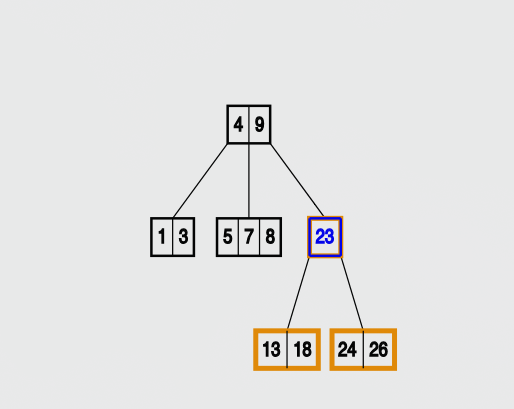
\includegraphics[scale=0.5]{figures/insertion4.png}
\end{figure}

Entretanto tal estrutura aumenta desnecessariamente a altura da árvore, isso pois o nó pai no "singleton" 23 ainda pode comportar elementos. Sendo assim ele é alocado nele.

\begin{figure}[H]
	\centering
	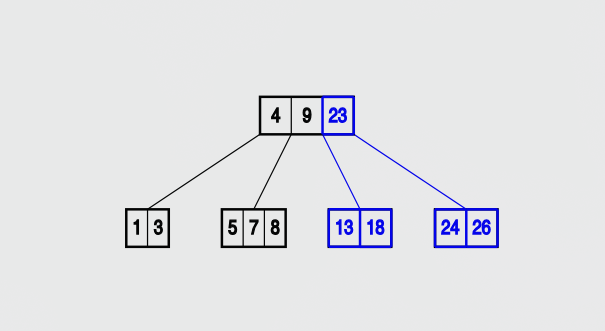
\includegraphics[scale=0.5]{figures/insertion5.png}
\end{figure}

Note que essa inserção causou mudanças estruturais mais significativas na árvore. E vale a pena lembrar que não necessariamente esse processo de para no nó imediatamente acima, tal processo pode se repetir sequencialmente até a raiz da árvore.

\section*{Remoção}
O processo de remoção é a operação mais complicada, tal complexidade é fruto da não violação das propriedades, bem como na inserção. As árvores usadas para exemplificação tem ordem 3. E a operação pode ser dividida em 3 cenários

\subsection*{Remoção em folha com mais de t elementos}
Se trata do melhor cenário, em que nenhuma mudança brusca vai acontecer na estrutura da árvore, isso pois como $n \geq $(t+1), sendo \texttt{n} o número de chaves no nó e \texttt{t} a ordem.

\begin{figure}[H]
	\centering
	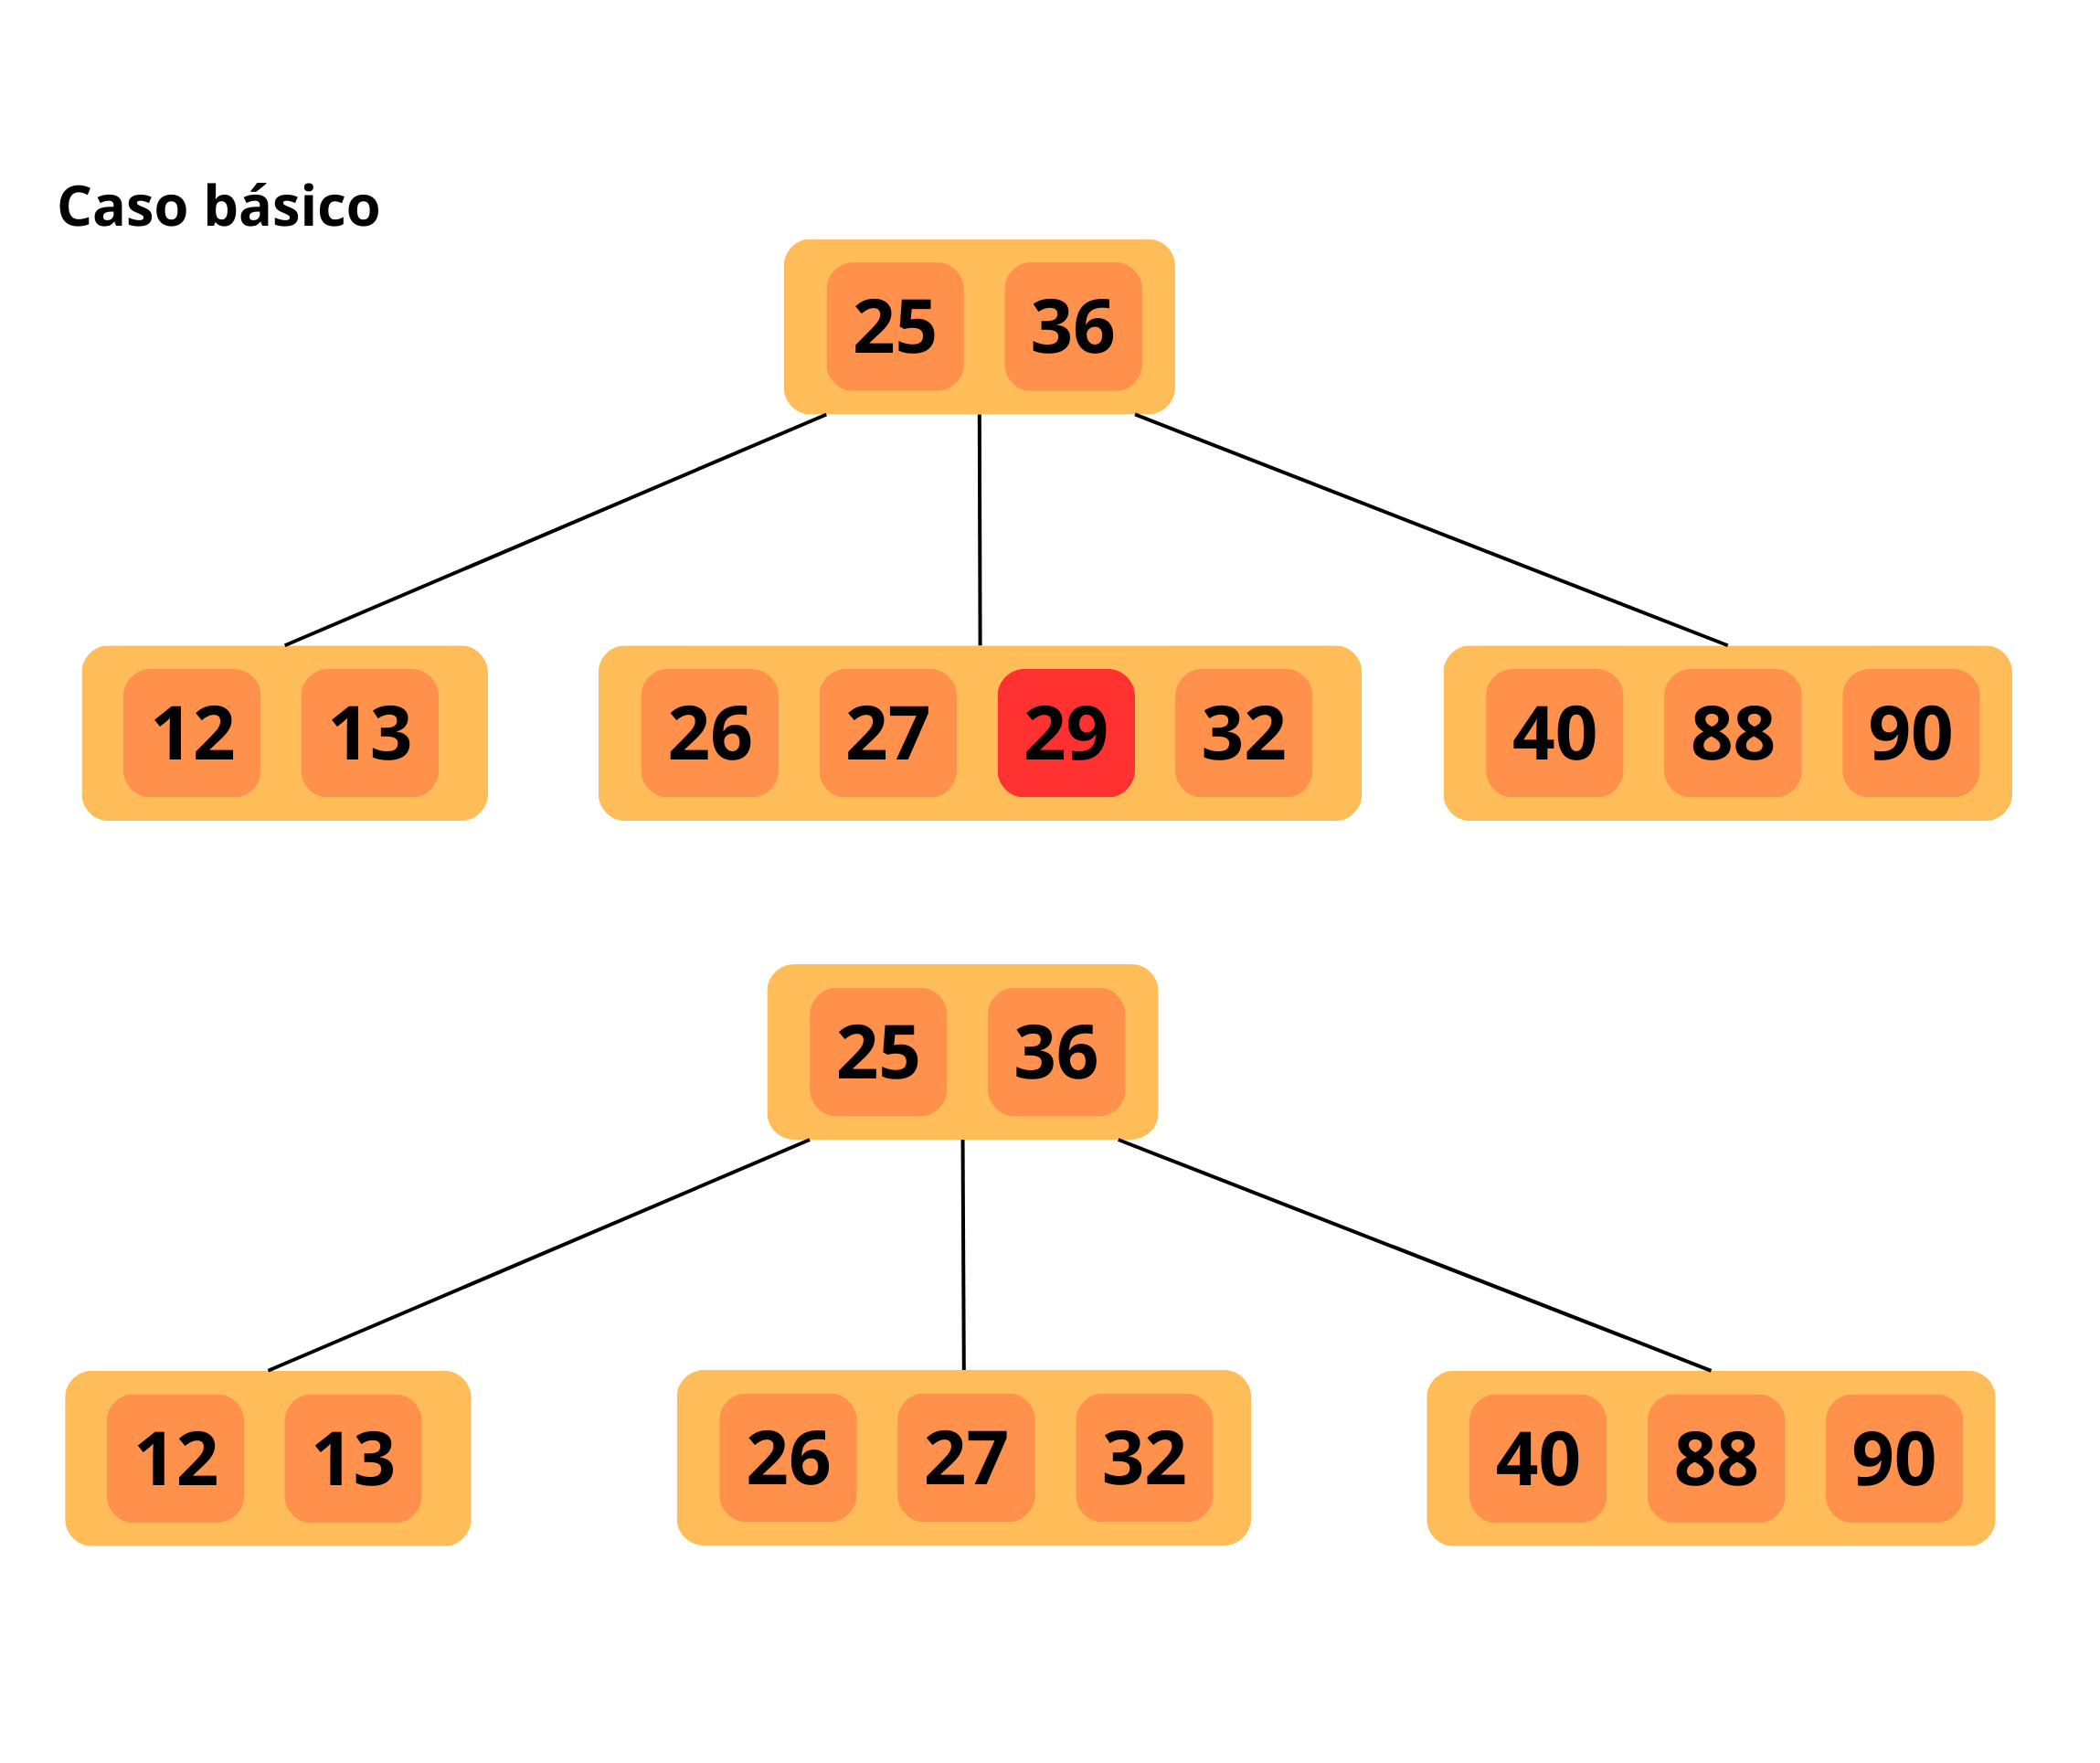
\includegraphics[scale=0.2]{figures/remocao1.png}
\end{figure}

Note que o elemento 29 foi excluído sem muito trabalho, isso pois seu nó tinha 4 elementos, e $4 \geq t+1$.

\subsection*{Remoção em nó não folha}

Este caso requer um pouco de atenção, pois é muito fácil violar $n \geq (t+1)$ se tratanto de um nó que não é folha. Muitas vezes será necessária uma realocação de elementos. O que na maioria dos casos vai implicar em no maior elemento do nó filho subir para a posição do pai excluído. Repare que isso acontece no exemplo abaixo

\begin{figure}[H]
	\centering
	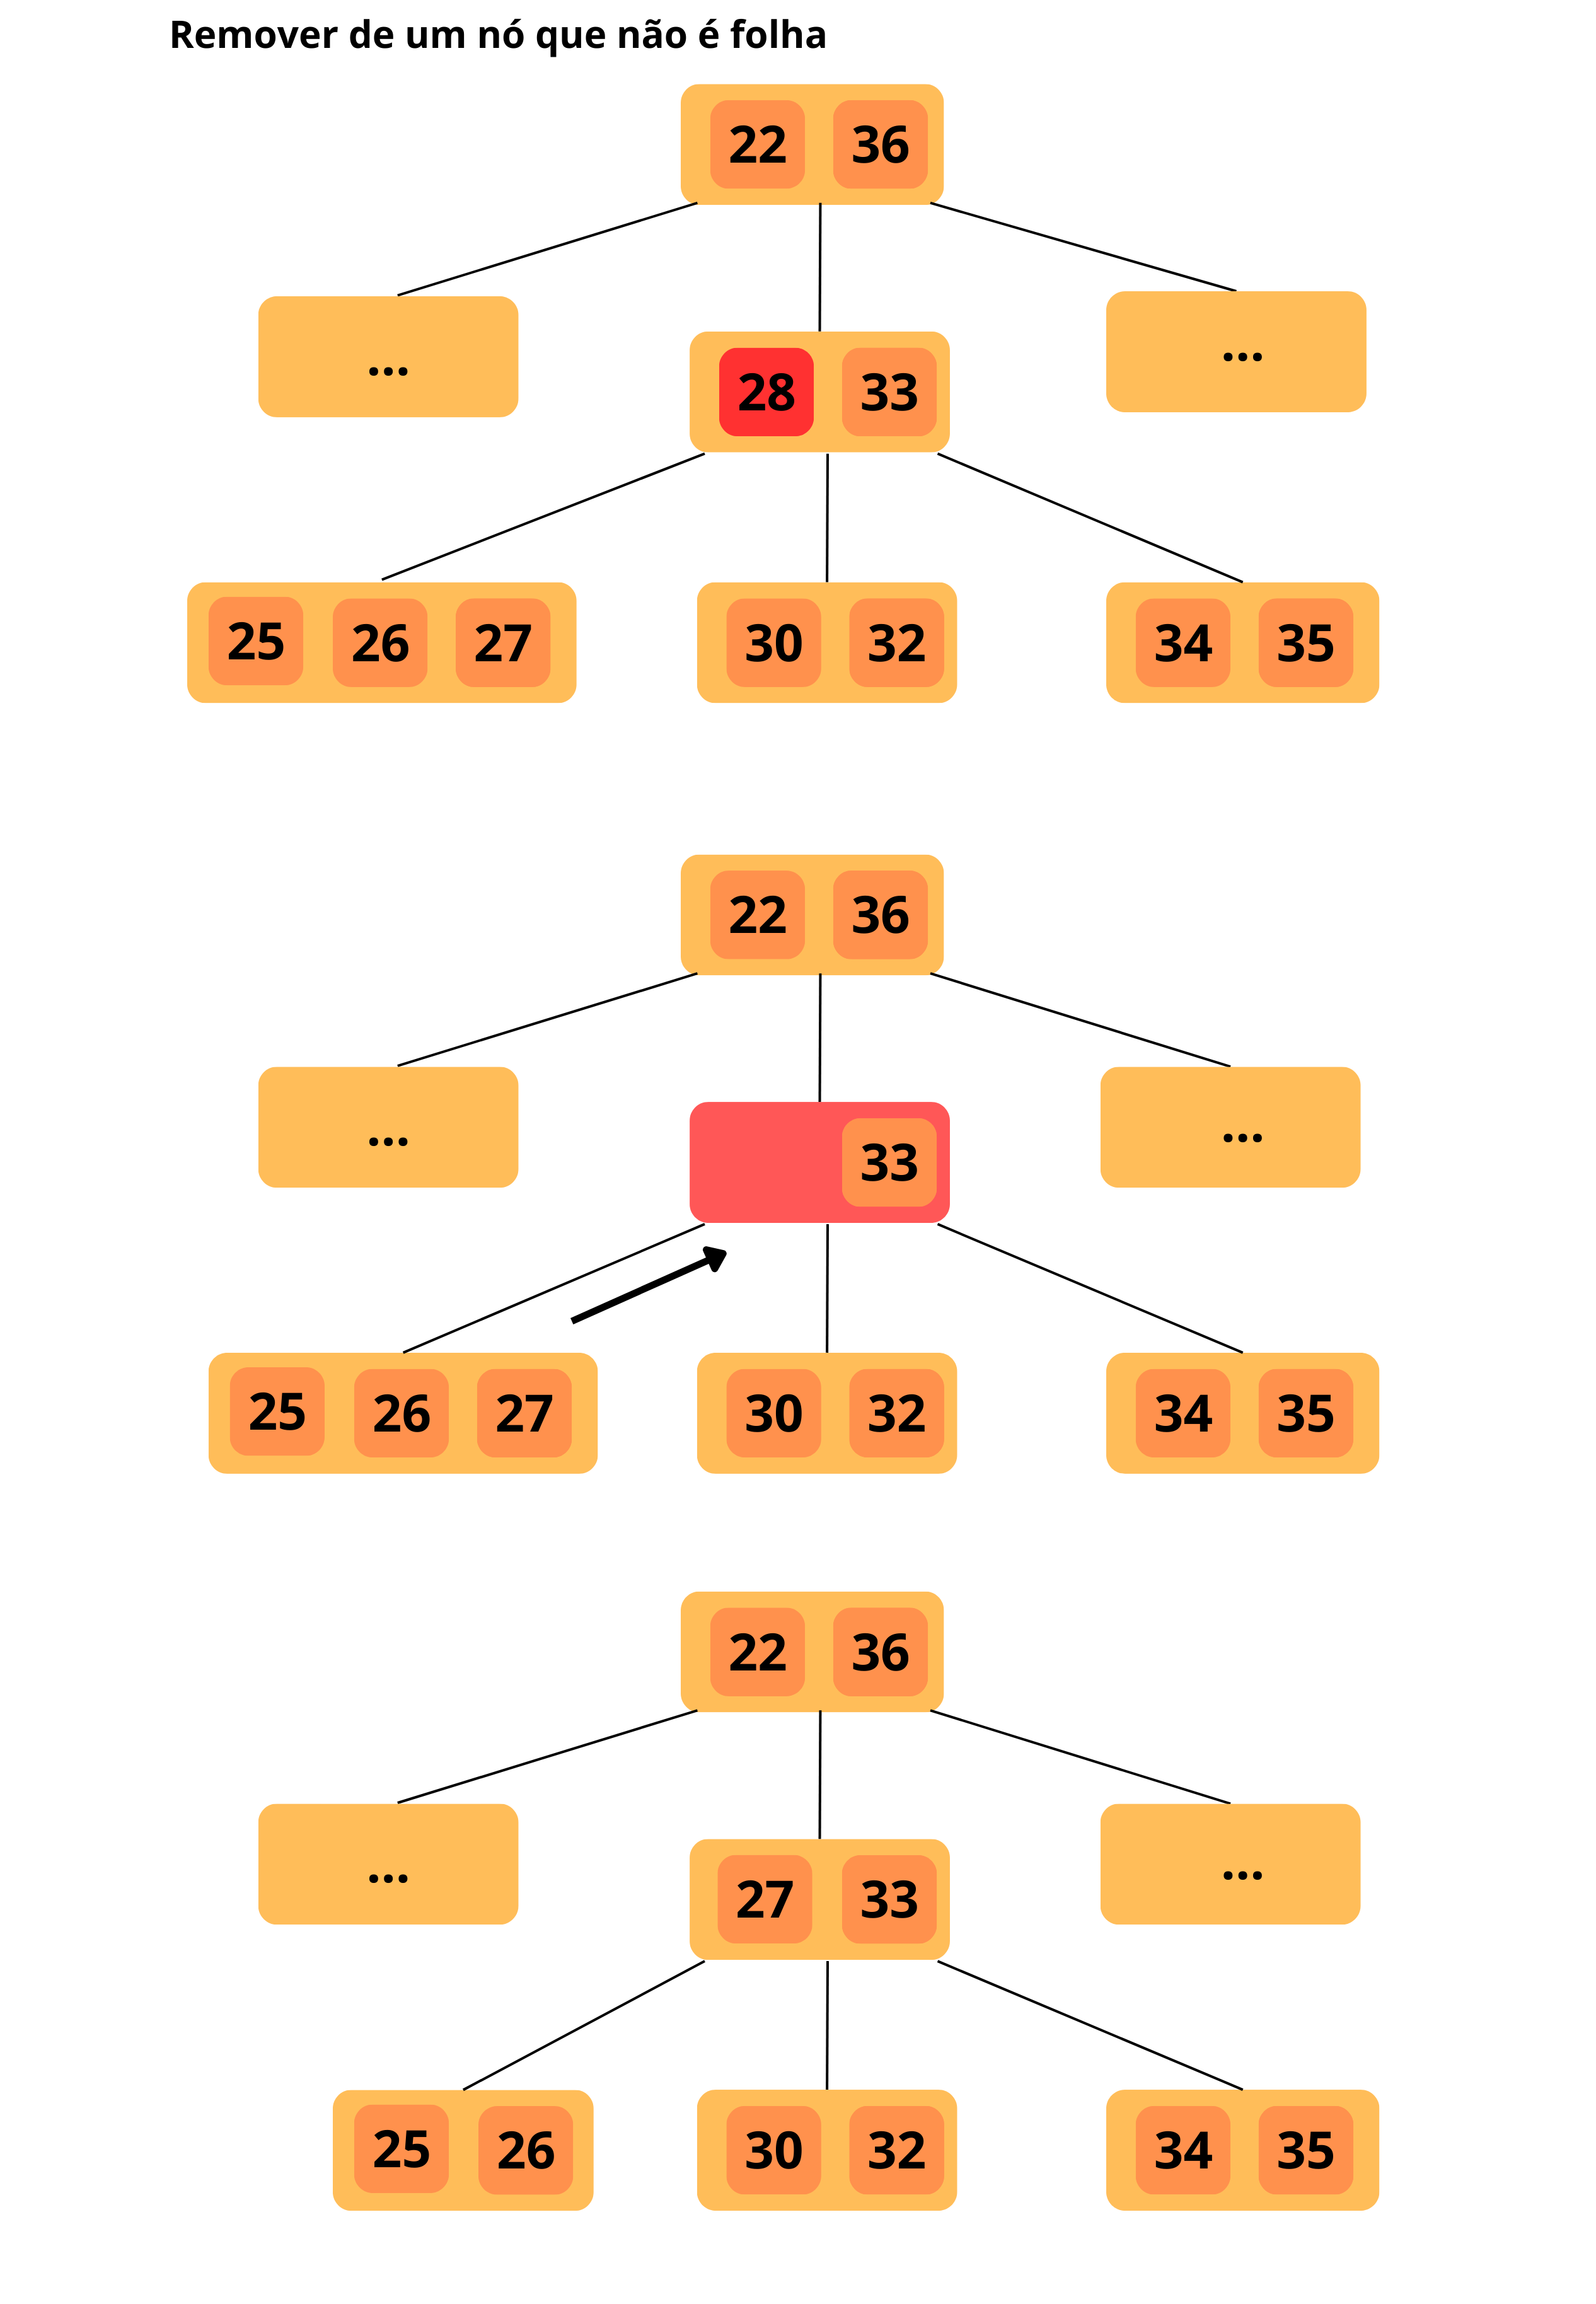
\includegraphics[scale=0.2]{figures/remocao4.png}
\end{figure}

A exclusão do 28 acarreta na violação da propriedade citada, sendo assim se faz necessário a alocação de um elemento para ocupar a posição do 28. O que faz com que o 27(maior valor no nó filho que o ponteiro a esquerda do 28 apontava) tome a posição do elemento excluído no nó pai. Também é importante se atentar que tal cenário não faz com que o nó filho viole a propriedade dado a realocação de um de seus valores chave.

\subsection*{Remoção em folha com t elementos}

Este último caso são particularizações do cenário acima, que na verdade dizem respeito a dois casos. Um em que os irmãos adjacentes somam mais de 2t chaves, e outro caso em que somam menos. \\

\textbf{Exclusão em um nó cujos irmãos adjacentes somam menos de 2t} \\

Sendo o alvo da exclusão o 22, perceba que o seu nó tem apenas um nó irmão adjacente, e este tem apenas 2 elementos, sendo assim $2 < 2t$.

\begin{figure}[H]
	\centering
	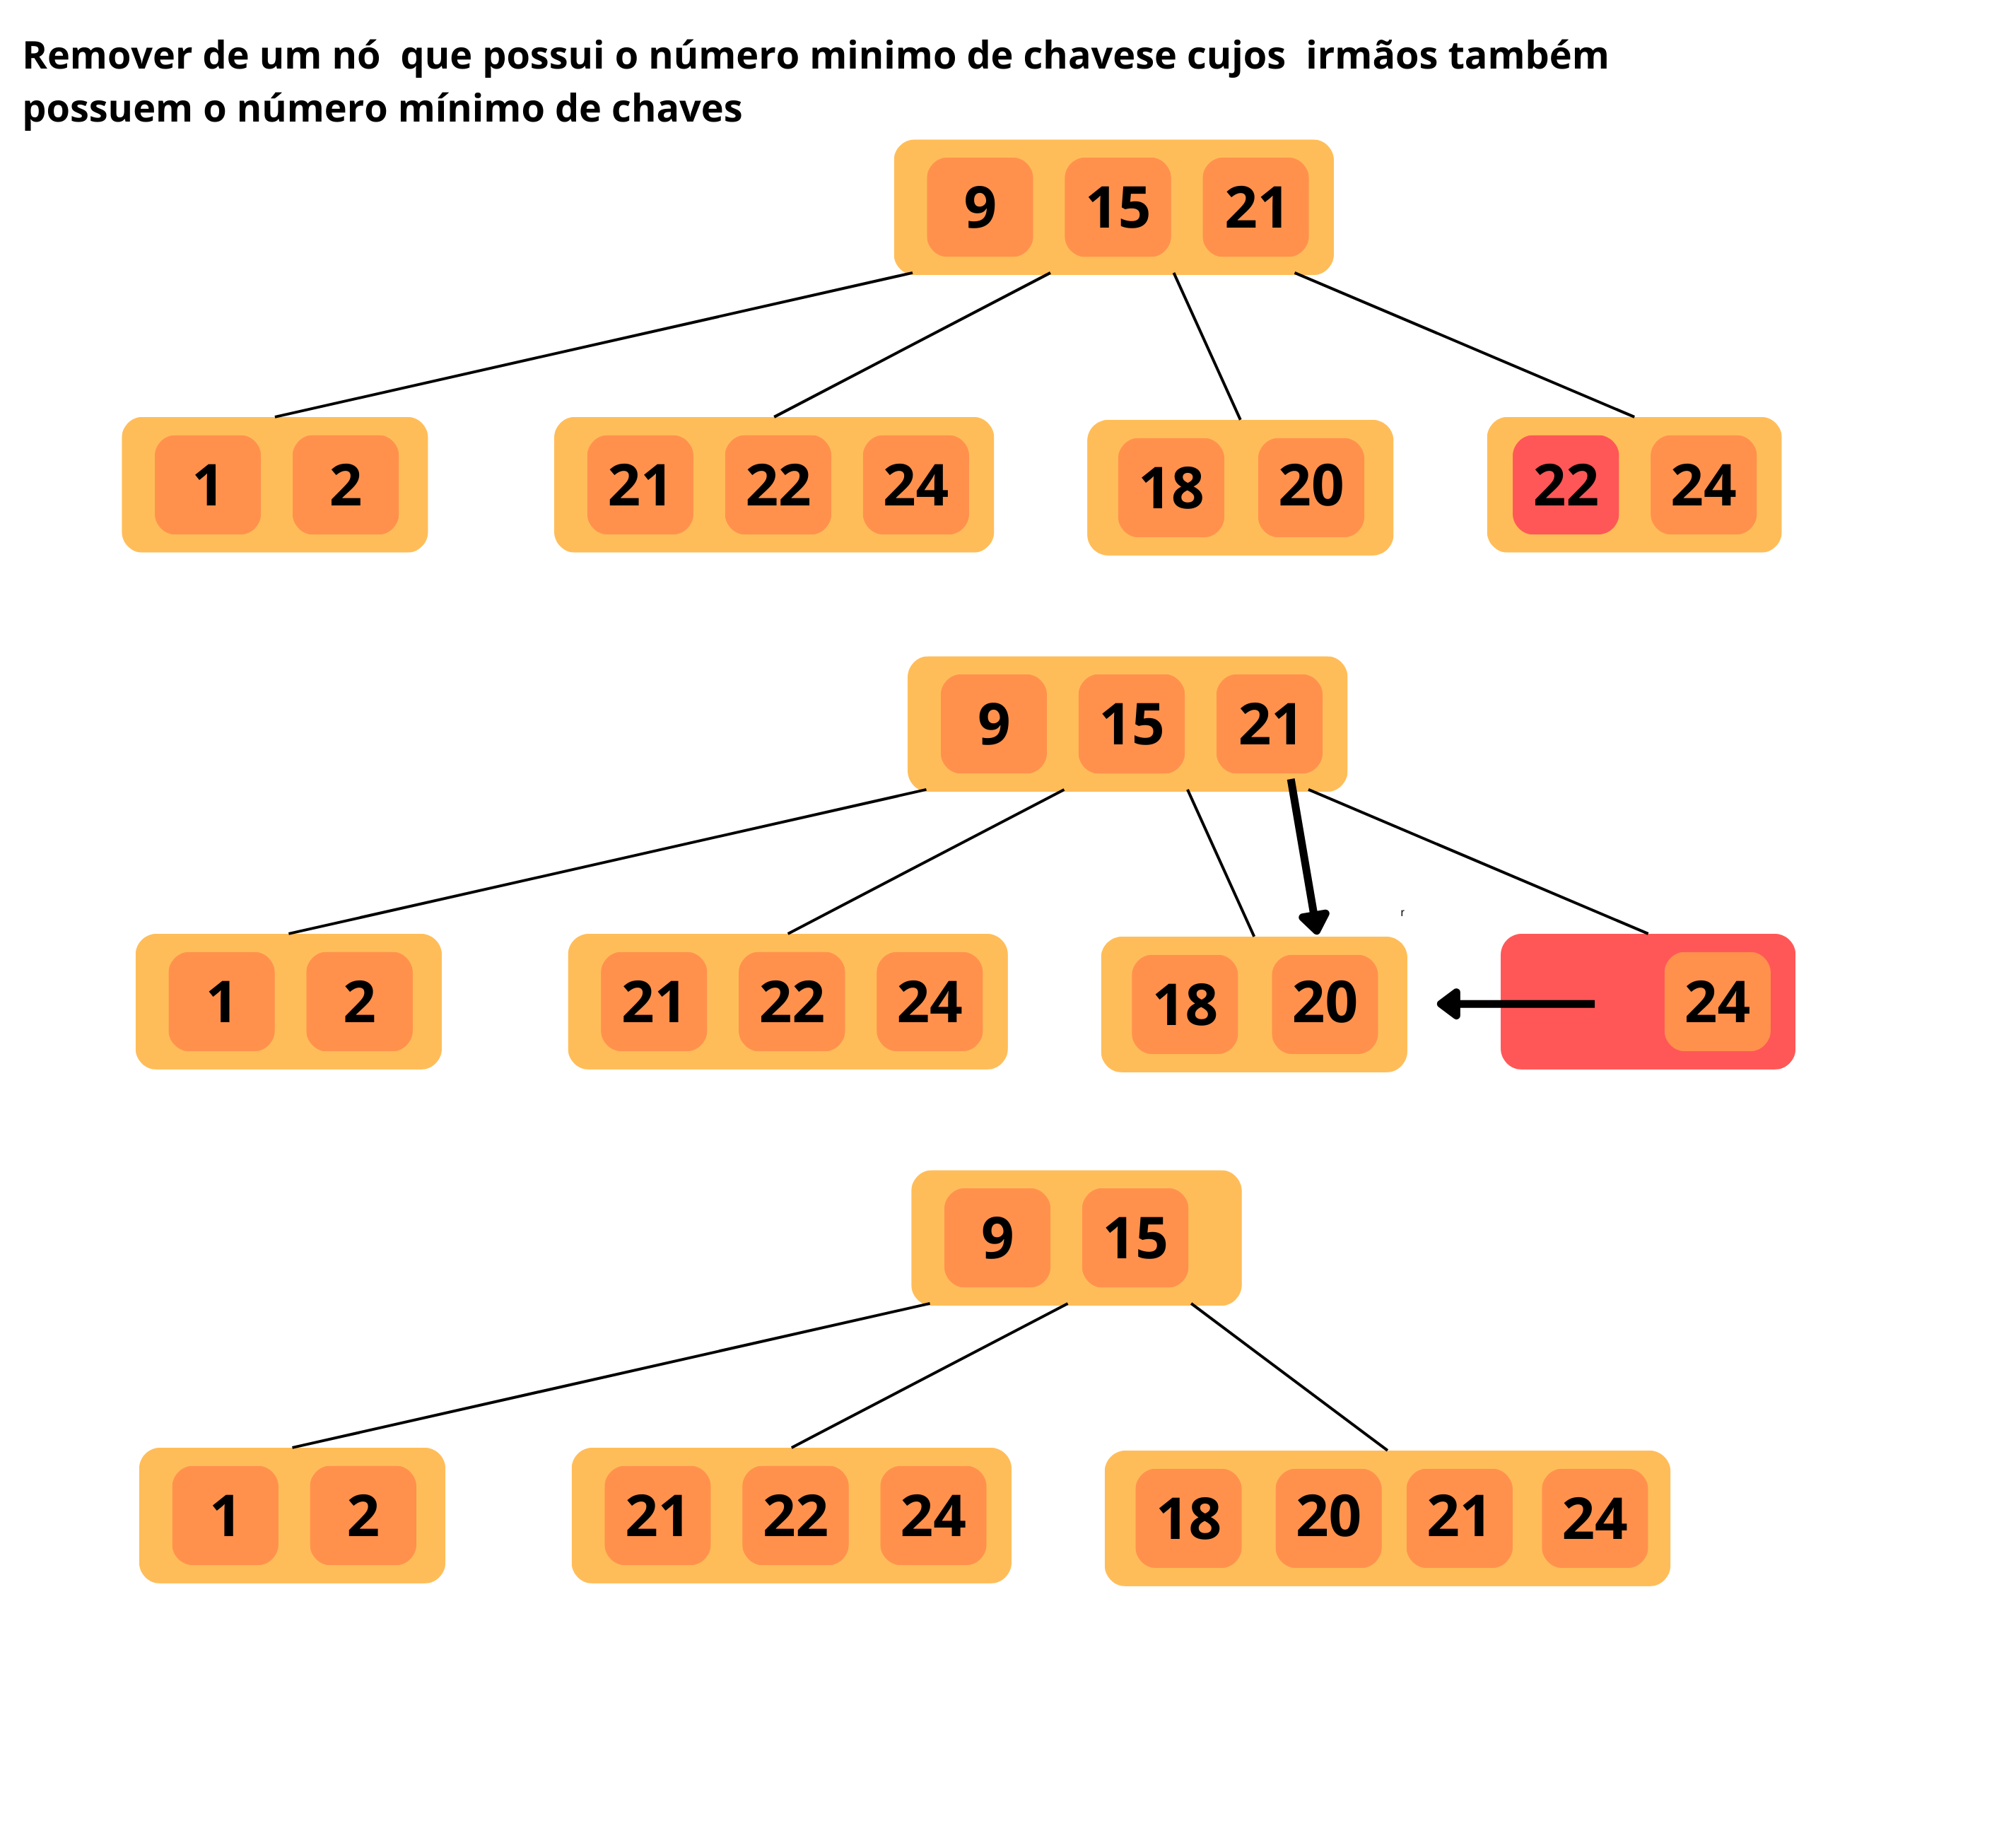
\includegraphics[scale=0.2]{figures/remocao3.png}
\end{figure}

Note que ao excluí-lo, seu nó viola o mínimo necessário de elementos. Sendo assim ele é realocado para o nó vizinho. Entretanto ao fazer isso o nó pai fica com um ponteiro desnecessário, pois só havendo 3 filhos só se faz necessário 2 elementos no nó pai(ou seja, 3 ponteiros). Isso acarreta na descida do 21 para o nó recém-formado, de forma que essa realocação não viola o número máximo de elementos possível.\\

\textbf{Exclusão em um nó cujos irmãos adjacentes somam 2t ou mais} \\

Perceba que no caso abaixo o 16 é o alvo da exclusão, entretanto, seus nós irmãos adjacentes somam 6 elementos e temos que $6 = 2t$. Sendo assim podemos fazer uma realocação razoavelmente simples dos elementos vizinhos para balancear a árvore.

\begin{figure}[H]
	\centering
	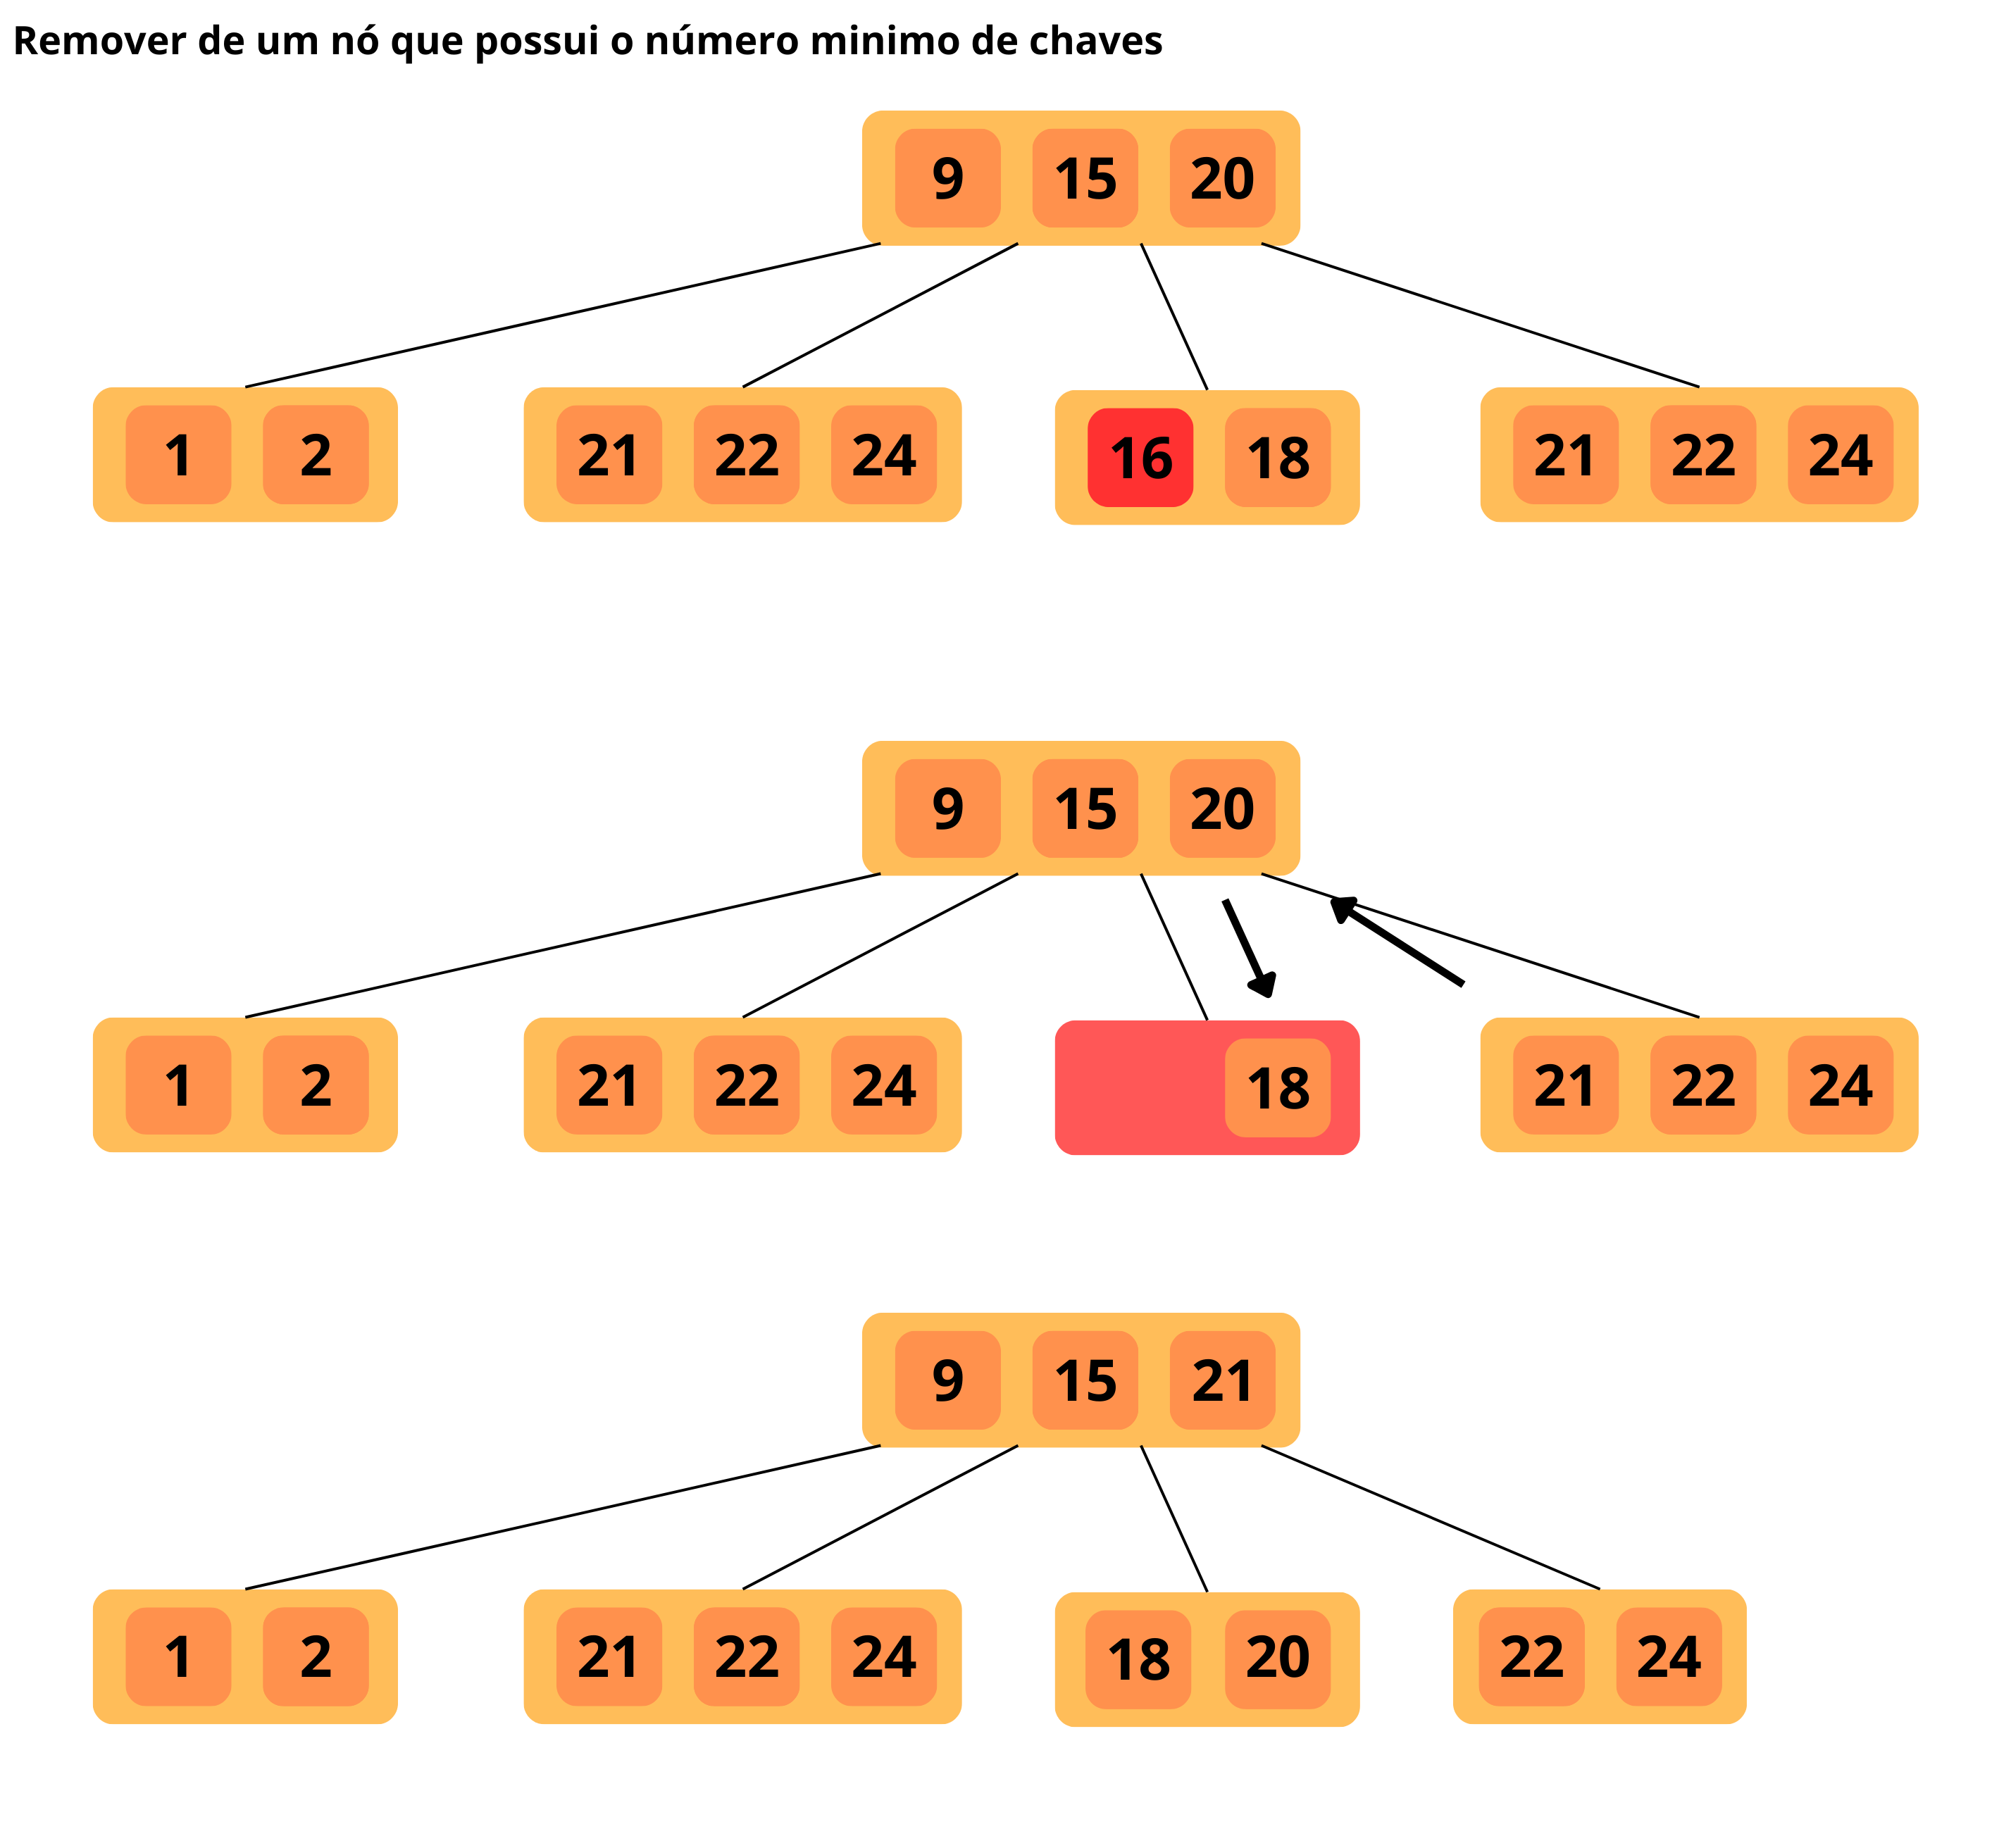
\includegraphics[scale=0.2]{figures/remocao2.png}
\end{figure}

Note que quando ocorreu a exclusão do 16 seu nó violou a propriedade do mínimo de elementos necessários. Sendo assim o 20 que estava no nó pai acabou descendo para compor o seu nó, e o 21 que era o menor element do irmão adjacente subiu para a posição onde antes estava o 20.
% \newpage
%


% -------------------------------------------------------------------
% Bibliography/References  -  Harvard Style was used in this report
% -------------------------------------------------------------------

\nocite{*}
\bibliographystyle{agsm} % Harvard Style 
\bibliography{references}  %  Patashnik, O. (1988), BibTEXing. Documentation for general BibTEX users.


\end{document}
